% \subsection{A Running Example}
% \label{sec:problem:example}

\begin{figure}[!htp]
\centering
%
\subfloat[A simple crypto scheme]{ 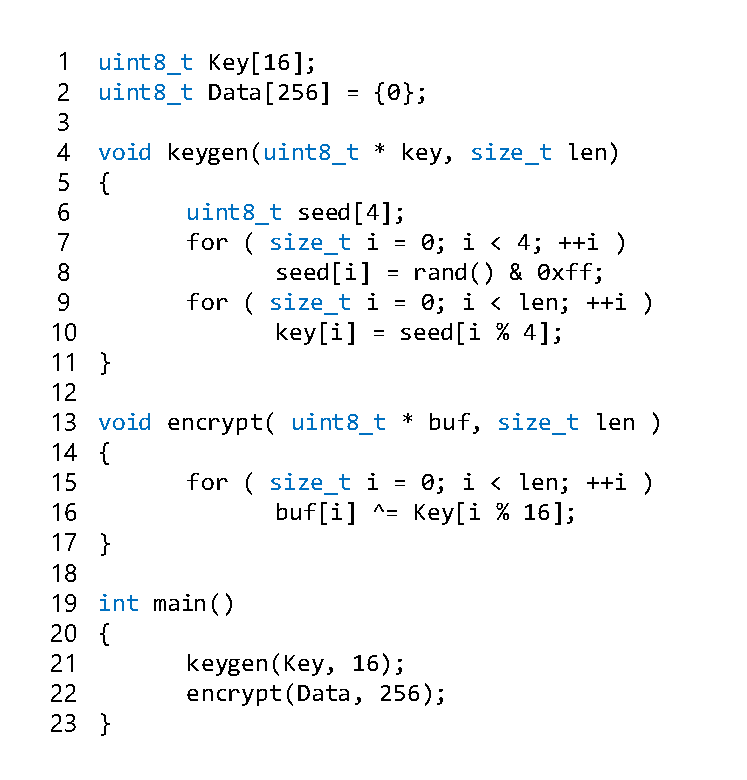
\includegraphics[width=0.4\textwidth]{code.pdf} \label{fig:dd:code} }

\subfloat[Partial corresponding disassembly code]{ 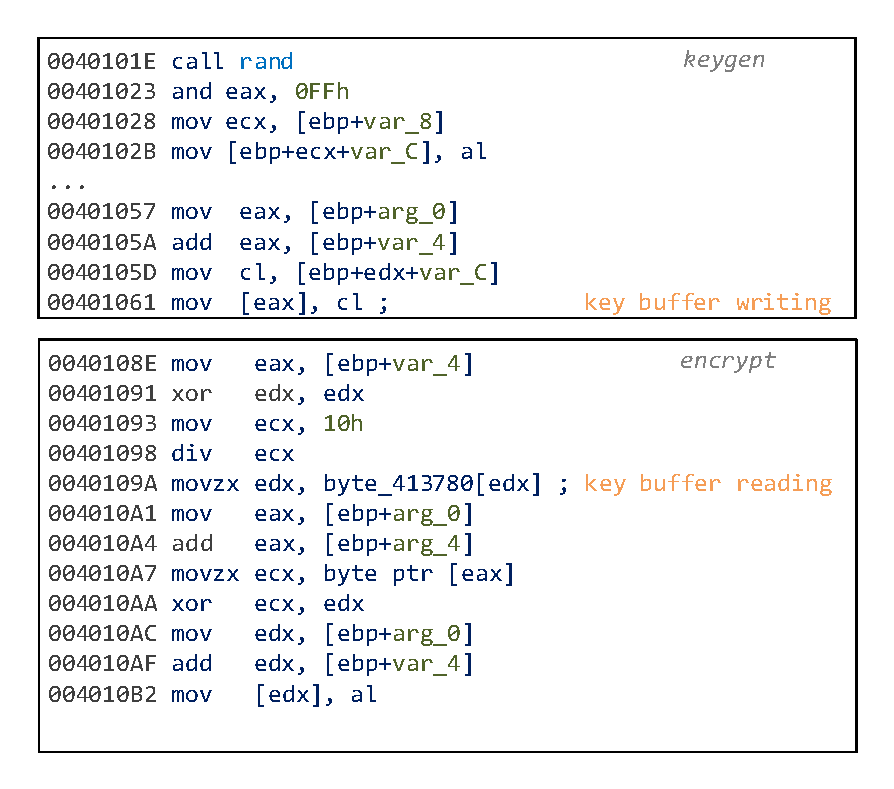
\includegraphics[width=0.4\textwidth]{depend.pdf} \label{fig:dd:asm} }
%
\caption{An example illustrating typically how a crypto key is used in a binary executable.}
\label{fig:dd}
\end{figure}

%\vspace{-0.15in}
%\paragraph{A Running Example} 
We use a simple but representative program, illustrated in~\autoref{fig:dd}, to demonstrate how our insecure crypto key detection works. 
This simple program encrypts \texttt{Data} 
%(defined at line 2 at Figure~\ref{fig:dd:code}) 
through masking a \texttt{Key} generated by the \texttt{keygen} function. 
The program captures a crypto operation (a simple cipher that mixes \texttt{Key} and \texttt{Data}) and a crypto key management (a home-made key derivation that generates a random key). 
{It has an insecure crypto key because 1) the key only contains four bytes of randomness and 2) the key is not sanitized after the encryption}.

To detect the insecure crypto key in this running example, a security analyst would need to 
(1) find which code blocks are crypto related; 
(2) identify the crypto key used by those blocks; 
(3) check how the identified crypto key is generated, i.e., which data sources affect it and how it is derived from those key materials; and
(4) monitor key propagation (i.e., the memory buffers that store the key) to check whether it is still available after the crypto operation. 
\sysname is designed to automate these steps with a principled approach. 

\paragraph{Challenges} 
To detect insecure keys using the above steps, our approach needs to address the following challenges:
\begin{compactitem}
\item \textbf{How to identify crypto operations without signatures}. 
Previous works that analyze crypto software often rely on signatures for specific crypto algorithms. 
Thus, if the algorithm is proprietary, the identification would fail, as no signatures would typically be available. 
In Figure\autoref{fig:dd:code}, the simple, home-made crypto operation cannot be identified with signatures. 

\item \textbf{How to identify the crypto keys}.
Even when the crypto operation has been identified, how to accurately locate the memory buffer that contains the crypto key is still non-trivial. 
For instance, the \texttt{encrypt} function in Figure\autoref{fig:dd:code} accesses two buffers: \texttt{Data} and \texttt{Key}. 
Unfortunately, when analyzing binary executables, there is no semantic information available on the buffers. 
Thus, our approach must identify which buffer is the crypto key buffer. 

\item \textbf{How to detect insecure crypto keys in complex programs}.
Having identified the buffer holding a key, we still need to determine if the key is correctly derived and managed. 
Unfortunately, programs that contain crypto algorithms are often complex and these algorithms usually only occupy a very small percentage of the entire program. 
It is infeasible and ineffective to analyze the whole program executable. 
Thus, we have to design an efficient way for detecting insecure crypto keys.
\end{compactitem}

% \begin{figure*}[!htbp]
% \centering
% 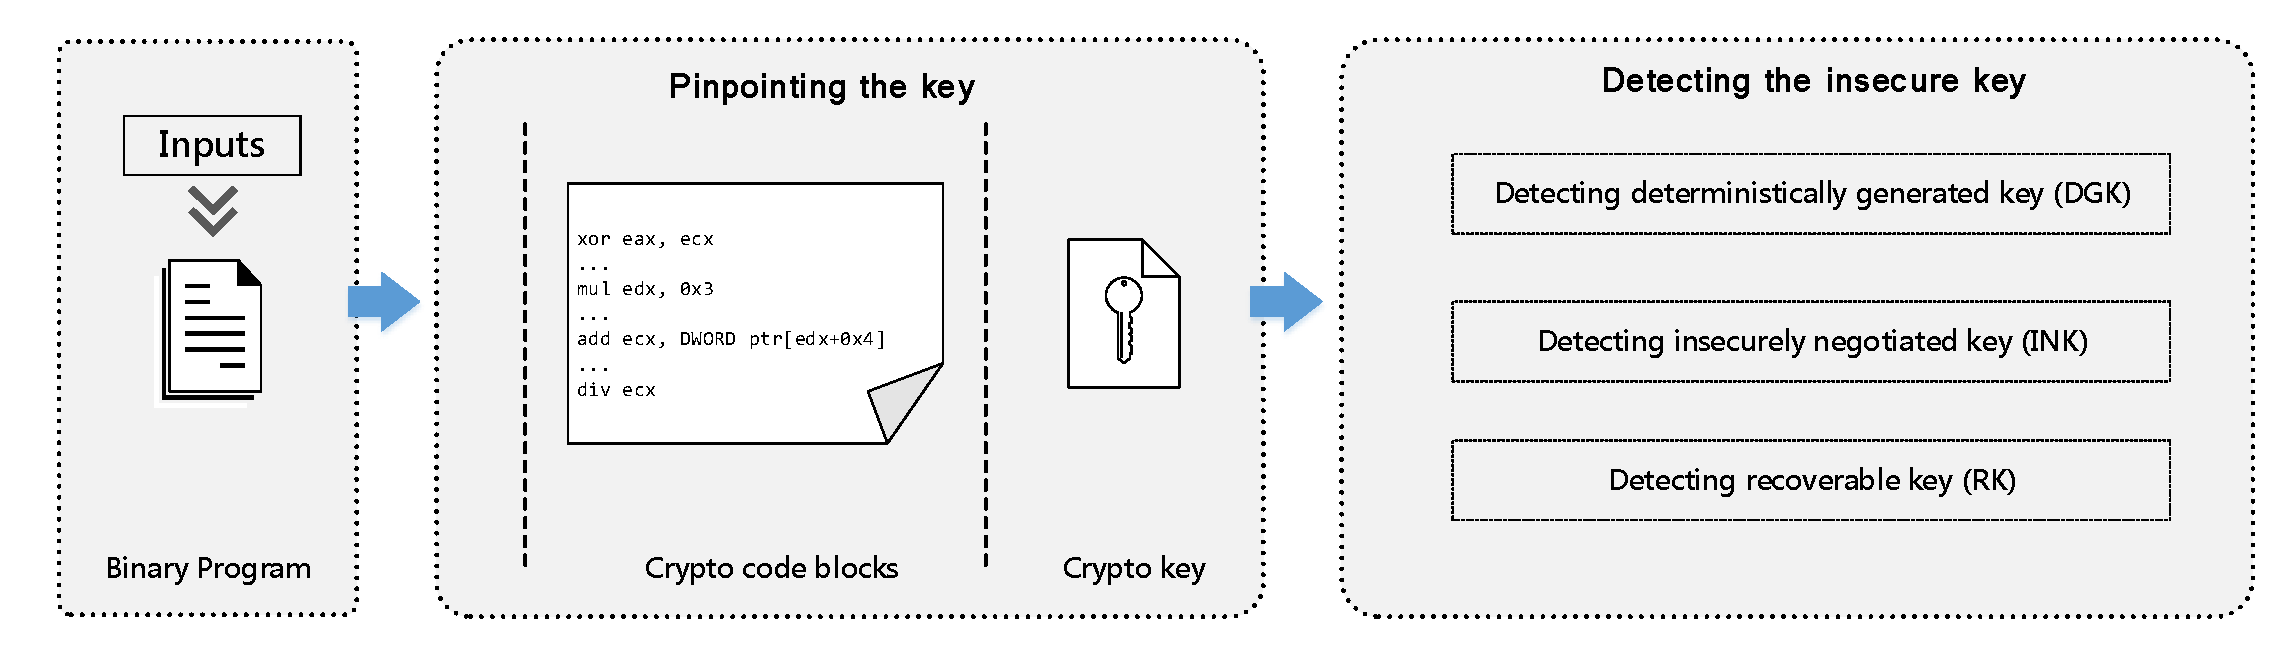
\includegraphics[width=0.9\textwidth]{flow.pdf}
% \caption{An Overview of \sysname.}\label{fig:workflow} 
% \end{figure*}


\paragraph{Insights} Fortunately, all of the challenges listed above can be solved with the following key insights:

\begin{compactitem}
\item
\textbf{Identifying crypto operations independent of their implementation}. 
Oftentimes, crypto operations are identified by scanning the implementation with signatures of well-known crypto algorithms. 
However, such approach cannot detect propietary algorithms.  
Instead, our approach identifies the {crypto basic blocks} at the core of the crypto operation. 
For this, it uses a dynamic analysis technique that leverages the insight that these core basic blocks usually mingle crypto keys and data, and thus have distinct properties. 
For instance, as shown in Figure~\ref{fig:dd:code}, the key masking operation (at line 16) reads from two data buffers and produces the ciphertext. 
Such crypto basic blocks have distinguishable properties such as high use of arithmetic instructions, producing data streams with high randomness, and having execution length proportional to the input size. 
If a basic block meets these three constraints, it is very likely that it is a crypto basic block.
% We can therefore rely on such features to find {crypto basic blocks} and further locate crypto keys. 
%We have to note that we are not the first to utilize this insight and it has been exploited before by Dispatcher~\cite{caballero2009dispatcher} and ReFormat~\cite{wang2009reformat}.

\item
\textbf{Locating the crypto keys}.
Once the core {crypto basic blocks} are identified, our approach then examines the data accessed by those blocks. 
Typically, {a crypto basic block} will process two inputs. 
For encryption, the plaintext and the key. 
For decryption, the ciphertext and the key. 
And, for digital signatures, the input message and the key. 
Note that while the verify function of a digital signature takes three inputs (message, key, signature), only the message and the key are used in the crypto operations.
Therefore, in all three cases we need to separate the crypto key from the other input. 
Interestingly, we notice that the size of the crypto key is usually very small (e.g., 128-bit) compared to the plaintext, ciphertext, or message, which could be of arbitrary length. 
We also observe that the crypto key and the other input are usually stored at different memory buffers. 
And, those buffers are usually filled with content derived from different data sources, e.g., a pseudo-random generator for keys and the network or the filesystem for the plaintext/ciphertext/message. 
%For instance, as shown in Figure~\ref{fig:dd:asm}, the operated crypto key and plaintext (line 7) depends on the memory writing operations at line 13 and 16, respectively. 

\item
\textbf{Detecting the insecure crypto keys}.
Since it is very complex to analyze the entire program to understand the handling of crypto keys, we instead propose a key-centric strategy. 
Having identified the crypto operations and located the crypto keys, we use the identified keys as an index to further check the origin of each key and its propagation. 
For instance, through checking the origin of the key in~\autoref{fig:dd} we can find that it is generated from the \texttt{keygen} function at line 10, {and through checking the input of this function we can discover the crypto key buffer contains inadequate information (i.e., only 32 bits) }.
Moreover, by monitoring the key buffer we can observe that its content is preserved until the program terminates, and thus it is an insecure crypto key. 
This backward and forward key tracking hence provides a simple way to detect insecure crypto keys.
\end{compactitem}


\paragraph{Problem Scope}
The objective of this work is to identify  insecure crypto keys in binary executables.
In particular, we focus on detecting (1) whether the key is generated from deterministic inputs, (2) whether a shared key is generated using key materials from a single party, and (3) whether the key is not sanitized immediately after the cryptographic operations. 
%
We focus on analyzing x86/64 stripped executables without source code or debugging symbols. 
%Particularly, we focus on both situations where cryptographic code is statically linked into a host program (thus the symbol names are removed) or dynamically invoked as an independent library (thus the symbol names are kept for dynamic linking). 
%With respect to the insecure crypto keys,
In addition, we focus on ciphers (symmetric, asymmetric, stream) and digital signatures. 
For these classes of cryptographic primitives, it does not matter which specific crypto algorithm the program uses.
Thus, our approach handles both standard and proprietary algorithms.
Other cryptographic primitives such as hash functions do not use keys, or in the case of keyed hashes they do not apply the crypto operations on the input and the key simultaneously.
% , thus violating our insights.

